% \input{"IAB/latex/TeX-Folienformat.tex"}
\input{"/Users/jonathanlatner/Google Drive/My Drive/IAB/latex/TeX-Folienformat.tex"}

\documentclass[t,8pt,utfx8]{beamer}
\usepackage{booktabs}
\usepackage{setspace}
\usepackage{parskip}
\usepackage{graphicx}
\usepackage{subcaption}
\setbeamertemplate{caption}[numbered]
\newcommand{\sprache}{\englisch}
\renewcommand{\thesubsection}{\alph{subsection})}
\usepackage[cal=pxtx, scr=dutchcal]{mathalpha}
\usepackage{forest}



\definecolor{codegreen}{rgb}{0,0.6,0}
\definecolor{codegray}{rgb}{0.5,0.5,0.5}
\definecolor{codepurple}{rgb}{0.58,0,0.82}
\definecolor{backcolour}{rgb}{0.95,0.95,0.92}



\newcommand{\btVFill}{\vskip0pt plus 1filll}


\title{Buyer Beware: Understanding the trade-off between utility and risk in CART based models using simulation data}

\subtitle{Berlin, \newline 7-8. Oktober, 2024}

\author{Jonathan Latner, PhD \newline Dr. Marcel Neuenhoeffer \newline Prof. Dr. Jörg Drechsler}

\newcounter{noauthorlines}
\setcounter{noauthorlines}{2} % Wert für 2 Autoren über 2 Zeilen. Ggf. anpassen

% %%%%%%%%%%%%%%
% Ende Anpassung
% %%%%%%%%%%%%%%

% \input{"IAB/latex/TeX-Folienformatierung_CD_2019"}
\input{"/Users/jonathanlatner/Google Drive/My Drive/IAB/latex/TeX-Folienformatierung_CD_2019"}

% Modify the section in toc template to enumerate
\setbeamertemplate{section in toc}{%
    \inserttocsectionnumber.~\inserttocsection\par
}

% use for subsections
% \setbeamertemplate{subsection in toc}{}
\setbeamertemplate{subsection in toc}{%
    \setlength{\parskip}{1mm}
        \hskip2mm -- \hskip1mm\inserttocsubsection\par
}


\usepackage{colortbl}
\definecolor{lightgray}{gray}{0.9}

\usepackage{listings} %include R code
\lstdefinestyle{mystyle}{
    backgroundcolor=\color{backcolour},   
    commentstyle=\color{codegreen},
    keywordstyle=\color{magenta},
    numberstyle=\tiny\color{codegray},
    stringstyle=\color{codepurple},
    basicstyle=\ttfamily\tiny,
    breakatwhitespace=false,         
    breaklines=true,                 
    captionpos=b,                    
    keepspaces=true,                 
    numbers=left,                    
    numbersep=5pt,                  
    showspaces=false,                
    showstringspaces=false,
    showtabs=false,                 
    columns=fullflexible,
    frame=single,
    tabsize=2
}
\lstset{style=mystyle}


\begin{document}


\frame[plain]{\titlepage}

\begin{spacing}{1.25}


%%%%%%%%%%%%%%%%%%%%%%%%%%%%%%%%%%%%%%%%
%%%%%%%%%%%%%%%%%%%%%%%%%%%%%%%%%%%%%%%%
\section{Introduction}\label{sec:intro}
%%%%%%%%%%%%%%%%%%%%%%%%%%%%%%%%%%%%%%%%
%%%%%%%%%%%%%%%%%%%%%%%%%%%%%%%%%%%%%%%%

% \begin{frame}[c,plain]
% \vskip-4mm
% \begin{beamercolorbox}[wd=\boxwidth,ht=22.11mm]{transparent}%
%     \vfill%
%     \usebeamerfont{title}%
%     \leftinsert%
%     \MakeUppercase{Section \ref{sec:intro}: Introduction
% } % <- Hier die Überschrift eintragen
% \end{beamercolorbox}
% \vskip-3mm
% \pgfuseimage{rahmenlinie}
% \end{frame}


\frame{\frametitle{Overview}
\begin{itemize}
    \item It is well established that there is a trade-off between utility and privacy when generating synthetic data
    \item Utility in CART based synthesizers is high (Little et al., 2022; Danker and Ibrahim, 2021)
    \item Are CART based synthesizers actually preserving privacy?  If so, how?
    \item Using simulation data (Reiter et al., 2014), results suggest synthetic data from CART models are disclosive
    \item Disclosive in ways that are not observable using traditional privacy measures
\end{itemize}
}

\frame{\frametitle{Whats the goal of synthetic data?}
\begin{itemize}
    \item Synthetic data can accelerate development by replacing sensitive values with synthetic ones with minimal distortion of the statistical information contained in the original data set. (Jordan et al., 2022; Nowak et al., 2016)
    \item Low disclosure risk (R)
    \item High data utility (U)
    \item Visualize the trade-off using the R-U confidentiality map (Duncan et al., 2004)
\end{itemize}
}

\frame{\frametitle{Whats the problem?}
\begin{itemize}
    \item High data utility -- It must be similar to and different from the original data. 
    \begin{itemize}
        \item At the extreme, if the goal is high utility, why not just release the original data?
    \end{itemize}
    \item Low disclosure risk -- Synthetic data is not automatically private. 
    \begin{itemize}
        \item At the extreme, if the goal is low privacy risk, why should we release any data?
    \end{itemize}
    \item Many measures of utility and privacy exist
    \begin{itemize}
        \item Therefore, its not clear if data have high utility or low risk
        \item 2 problems
        \begin{itemize}
            \item More specifically, how can we map R-U trade-off if there are multiple measures of both?
            \item More generally, how do we know if the data have high levels of utility and low levels of privacy?
        \end{itemize}
    \end{itemize}
\end{itemize}
}


\frame{\frametitle{What do we know?}
\begin{itemize}
    \item Reiter (2005) suggested using sequential modeling with Classification and Regression Trees (CART). 
    \item Utility
    \begin{itemize}
        \item Drechsler and Reiter (2011) found that CART models offered the best results in terms of preserving the information from the original data.
        \item Other comparisons also found CART is superior (Little et al., 2022; Danker and Ibrahim, 2021)
    \end{itemize}
    \item Privacy
    \begin{itemize}
        \item Some evidence also suggests CART is superior (Little et al., 2022)
        \item However, other evidence indicates that CART-based synthesis simply replicates most of the original records (Manrique-Vallier and Hu, 2018)
    \end{itemize}
\end{itemize}
}

\frame{\frametitle{How does sequential modeling with CART? (Nowak et al., 2022)}
\begin{itemize}
    \item Consider as an example a default synthesis, i.e. synthesis with all values of all variables ($Y_1, Y_2,\dots, Y_p$) to be replaced. 
    \item The first variable to be synthesised ($Y_1$) cannot have any predictors and therefore its synthetic values are generated by random sampling with replacement from its observed values. 
    \item The second variable to be synthesized ($Y_2$) is generated using the fitted model and the synthesised values of ($Y_1$). 
    \item The third variable to be synthesized ($Y_3$) is generated using the fitted model and the synthesized values of $Y_1$ and ($Y_2$)
    \item The distribution of the last variable ($Y_p$) will be conditional on all other variables. 
\end{itemize}
}


\frame{\frametitle{How does CART work?}

\begin{figure}[h]
\centering
\begin{forest}
for tree={align=left}
[{var1=1\\100\%}
    [{var2=1\\46\%}
        [{var3=1\\20\%}
            [{var4=1\\7\%}]
            [{var4=0\\14\%}]
        ]
        [{var3=0\\26\%}
            [{var4=1\\14\%}]
            [{var4=0\\12\%}]
        ]
    ]
    [{var2=0\\54\%}
        [{var3=1\\27\%}
            [{var4=1\\14\%}]
            [{var4=0\\13\%}]
        ]
        [{var3=0\\14\%}
            [{var4=1\\13\%}]
            [{var4=0\\14\%}]
        ]
    ]
]
\end{forest}
\end{figure}

}


%%%%%%%%%%%%%%%%%%%%%%%%%%%%%%%%%%%%%%%%
%%%%%%%%%%%%%%%%%%%%%%%%%%%%%%%%%%%%%%%%
\section{Simulated data}\label{sec:data}
%%%%%%%%%%%%%%%%%%%%%%%%%%%%%%%%%%%%%%%%
%%%%%%%%%%%%%%%%%%%%%%%%%%%%%%%%%%%%%%%%
\frame{\frametitle{Simulate data with a unique record}
Borrowing from Reiter et al. (2014), we set the first 999 observations to be a random sample from a multinomial distribution for all combinations of $var1(0,1), var2(0,1), var3(0,1), var3(0,1)$ except (var1=1,var2=1,var3=1,var4=1), which we set to be the 1000th observation. 

\begin{minipage}{0.48\textwidth}
    \centering
    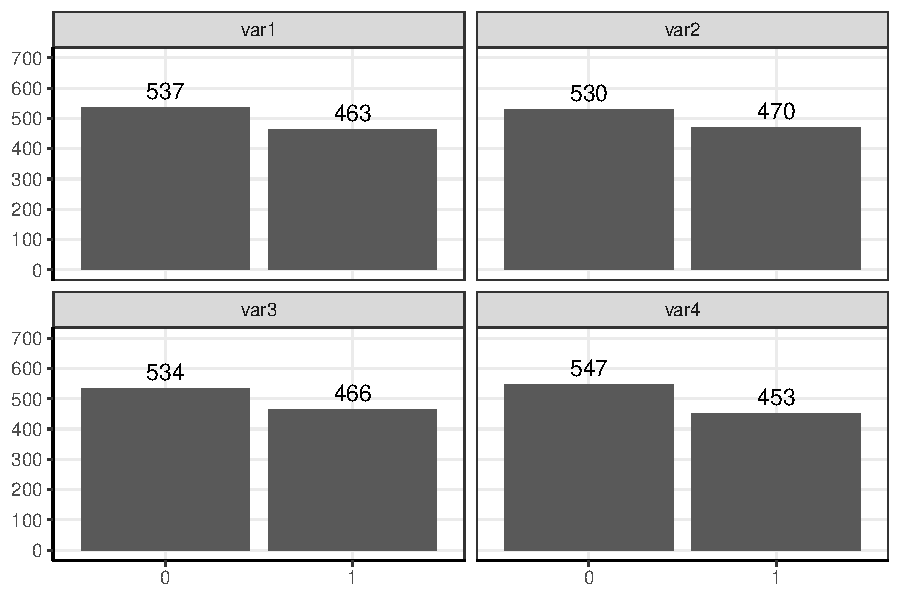
\includegraphics[width=\textwidth]{../../graphs/graph_numeric_frequency.pdf}
    \captionof{figure}{Frequency}
\end{minipage}
\hfill
\begin{minipage}{0.48\textwidth}
    \centering
    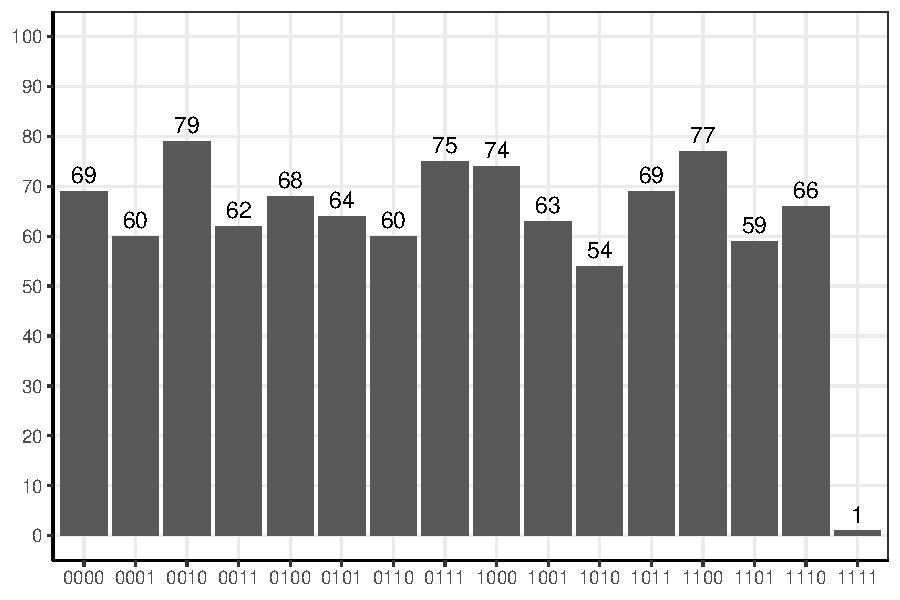
\includegraphics[width=\textwidth]{../../graphs/graph_numeric_histogram.pdf}
    \captionof{figure}{Histogram}
\end{minipage}

}

\frame{\frametitle{Simulate data with a unique record}

\begin{minipage}{0.48\textwidth}
    \centering
    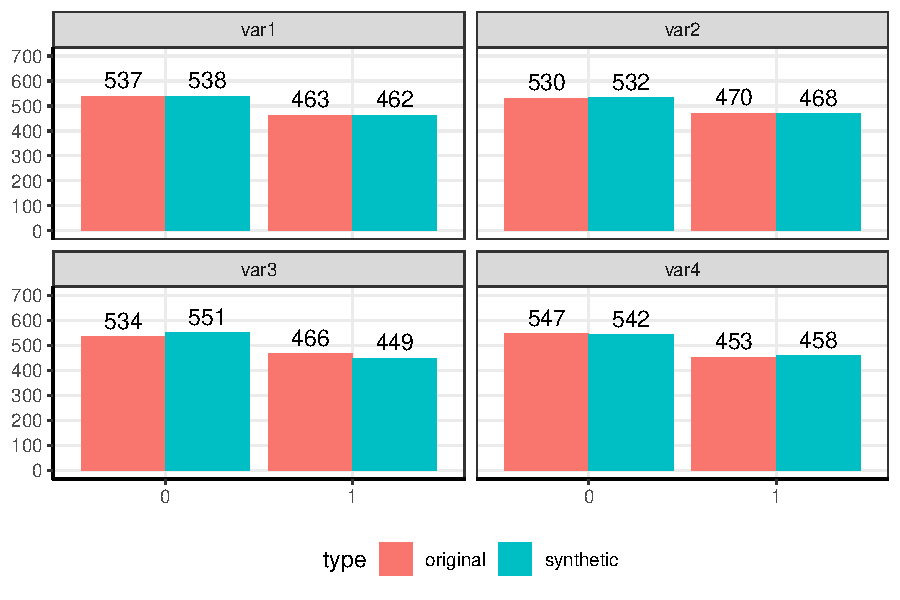
\includegraphics[width=\textwidth]{../../graphs/graph_numeric_compare_frequency.pdf}
    \captionof{figure}{Frequency}
\end{minipage}
\hfill
\begin{minipage}{0.48\textwidth}
    \centering
    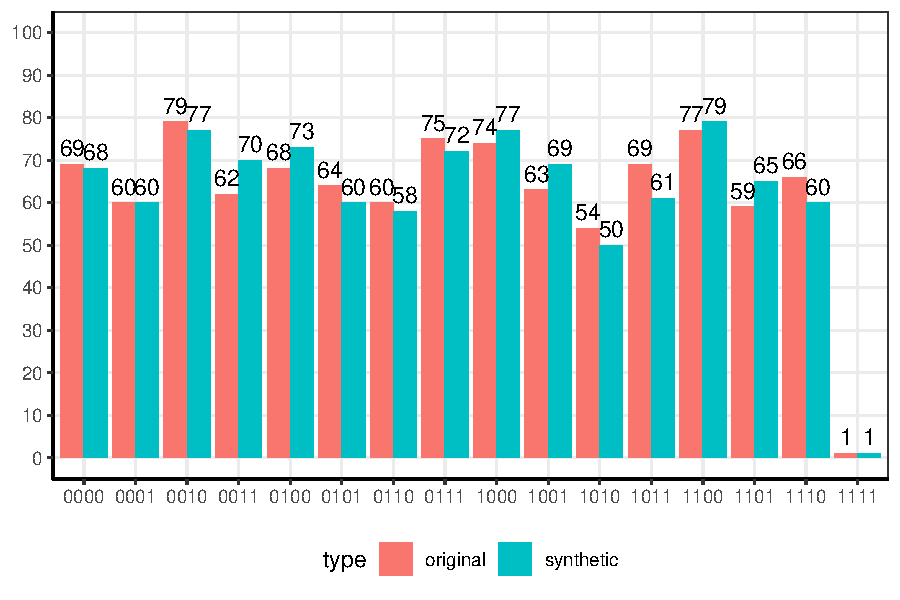
\includegraphics[width=\textwidth]{../../graphs/graph_numeric_compare_histogram.pdf}
    \captionof{figure}{Histogram}
\end{minipage}

}

\frame{\frametitle{Compare histogram x 100 synthetic datasets}
\begin{figure}
    \caption{}
    \resizebox{\textwidth}{!}{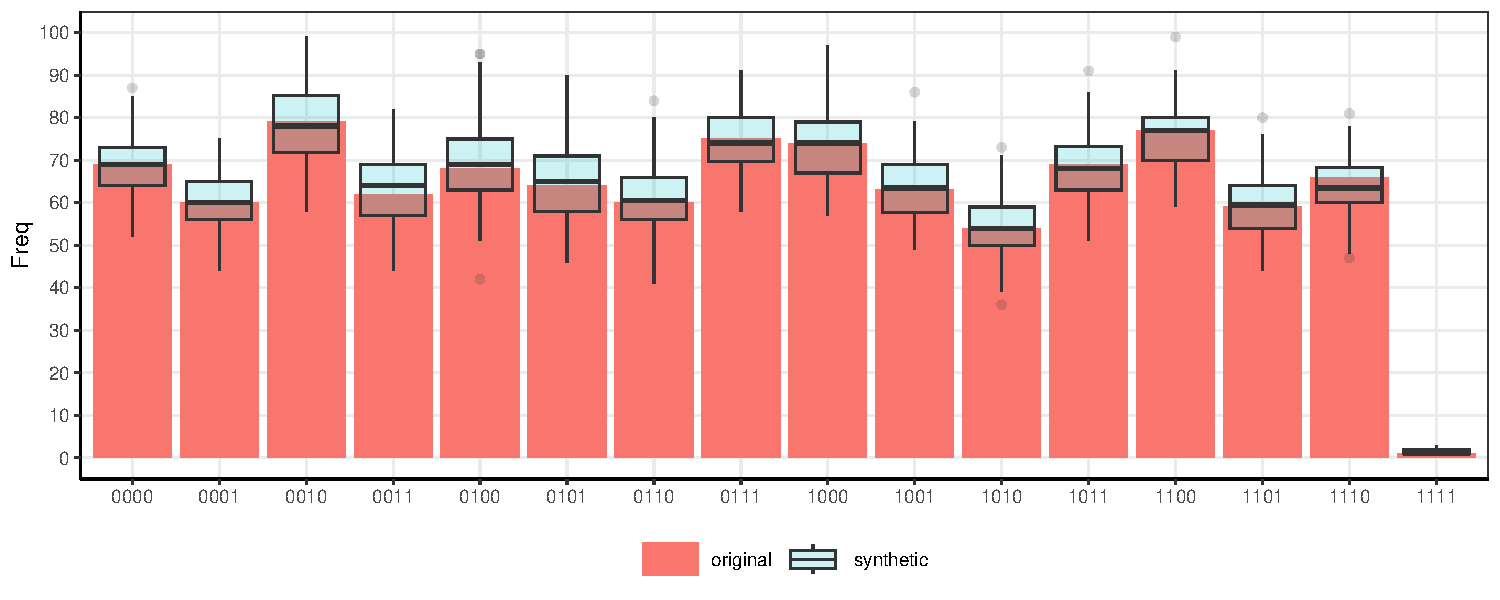
\includegraphics{../../graphs/graph_numeric_compare_histogram_100.pdf}}
    \label{fig:graph_numeric_compare_histogram_100}
\end{figure}
}

%%%%%%%%%%%%%%%%%%%%%%%%%%%%%%%%%%%%%%%%
%%%%%%%%%%%%%%%%%%%%%%%%%%%%%%%%%%%%%%%%
\section{Measuring utility and privacy}\label{sec:measuring}
%%%%%%%%%%%%%%%%%%%%%%%%%%%%%%%%%%%%%%%%
%%%%%%%%%%%%%%%%%%%%%%%%%%%%%%%%%%%%%%%%
\frame{\frametitle{Comparing utility measures}
all utility measures close to 0, i.e. high utility
}

\frame{\frametitle{Comparing privacy measures}
all privacy measures close to 0, i.e. low privacy risk
}

%%%%%%%%%%%%%%%%%%%%%%%%%%%%%%%%%%%%%%%%
%%%%%%%%%%%%%%%%%%%%%%%%%%%%%%%%%%%%%%%%
\section{Measuring utility and privacy}\label{sec:measuring}
%%%%%%%%%%%%%%%%%%%%%%%%%%%%%%%%%%%%%%%%
%%%%%%%%%%%%%%%%%%%%%%%%%%%%%%%%%%%%%%%%
\frame{\frametitle{Comparing utility measures}
all utility measures close to 0, i.e. high utility
}

\frame{\frametitle{Comparing privacy measures}
all privacy measures close to 0, i.e. low privacy risk
}


\end{spacing}
\end{document}

